\documentclass[12pt]{report}
\usepackage{graphicx}
\usepackage{float}
\graphicspath{ {images/} }
\usepackage[
backend=bibtex,
style=numeric,
citestyle=numeric,
sorting=none]
{biblatex}
\addbibresource{mybib}
\setlength{\parskip}{5mm}

\begin{document}

\title{OTP and AES: A historical transition between two systems of cryptography}
\author{Valdemar Thanner\\Kantonsschule Zug\\supervised by Mr. Bernhard Keller}
\maketitle

\tableofcontents

\chapter{OTP: The One Time Pad}

\section{What is a "One Time Pad"?}
When speaking about OTP, it is important to distinguish between its two meanings: On the one hand, it is a technique used to encrypt information. This technique requires one single key, used both to encrypt and decrypt the information. This key is also referred to as a one time pad; therefore, it is important to distinguish between the one time pad (a cryptographical technique) and a one time pad (a key which is used to encrypt and decrypt information).

The One Time Pad is largely derived from the Vernam cipher, which is named after Gilbert Vernam. The Vernam cipher utilized a perforated tape (one of the earliest types of data storage) as the secret key\cite{vernampatent}. Each bit of data was stored in the form of a hole punched into the perforated tape.

\begin{figure}[H]
\centering
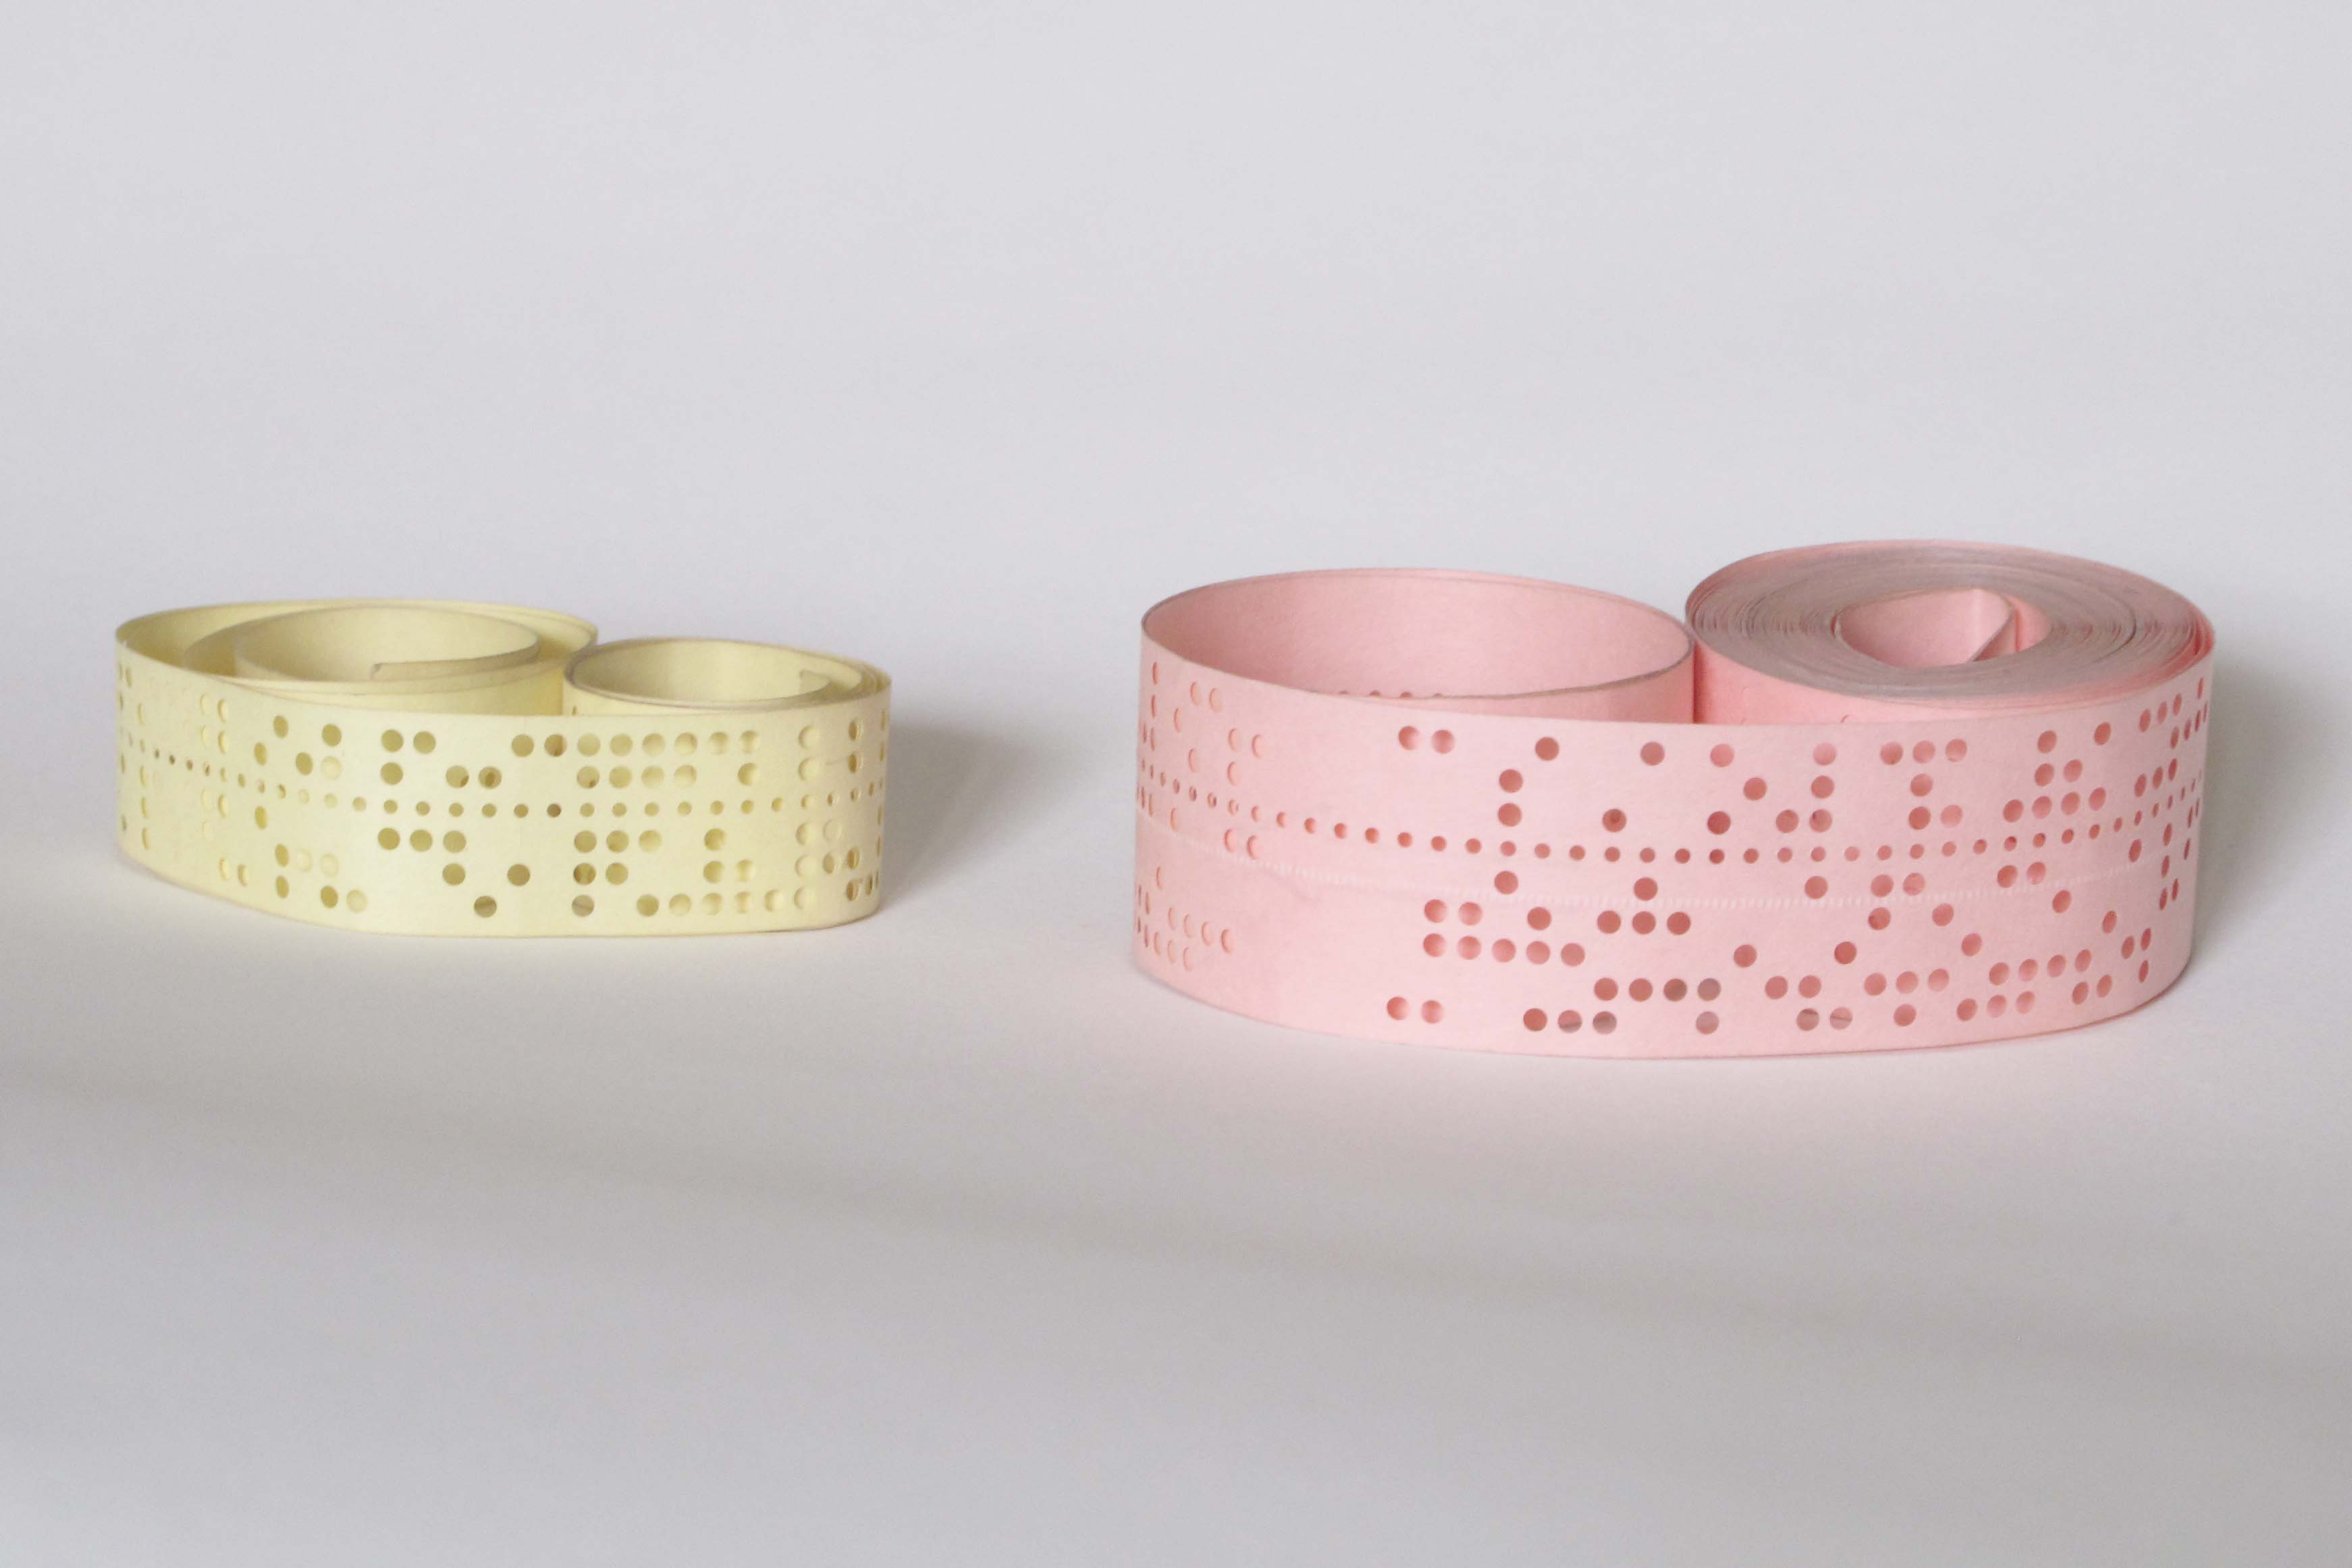
\includegraphics[scale=0.5]{PerforatedTape}
\caption{Perforated tape, utilized to store bits as punched holes}
\end{figure}

However, this system had a vulnerability which the One-Time Pad solved: In Vernam's original method, the perforated tape was not exchanged after it had completed one cycle; instead, it was looped around continuously, often being used to encrypt multiple different messages.

This made the entire system vulnerable. The re-usage of the key meant that the resulting ciphertext suffered from a so-called known-plaintext vulnerability \cite{HutSix}. This means that, if a plaintext and its corresponding ciphertext are captured, the key utilized to generate the ciphertext can be derived from them. This is not an issue if the key is exchanged each time a new message is encrypted. However, if the key of any Vernam cipher machine was compromised in this fashion, any further intercepted ciphertext could be decrypted.    

\section{Method used}
In the following section, the utilized method will be clarified through usage of an example. In this example, the message \textit{"cryptography"} will first be encrypted by it's sender, sent to it's intended recipient, and finally decoded by the recipient.

\subsection{Generation of the random key}
In order to encrypt the plaintext, a key must first be generated. This key will be utilized to encrypt the plaintext through the usage of modular addition, turning it into the ciphertext.

This key must fulfil some crucial criteria. Foremost, the length of the key (the amount of  characters contained within it) must be equivalent to or greater than the length of the plaintext; otherwise, it is not possible to perform any encryption (using the OTP). Secondly, the key must be generated randomly. This is mainly due to the fact that a randomly generated key makes frequency analysis\cite{frequencyanalysis}, the form of cryptanalysis most commonly used to break classical ciphers, impossible.

The key consists of numbers. Usually, when the plaintext is made up of Latin letters, the numbers range between 0 and 25. The key can be converted into Latin letters through the same method applied to the plaintext outlined in the following chapter, however, this is not necessary, although the key is often transported in the form of text.

As the message being encrypted in this example has 12 characters, the key must also posses at least 12 characters. For the sake of this example, the key \textit{"sytruifgnihm"} will be utilized.

\subsection{Modular addition of the key and plaintext}
Next, the ciphertext is created through modular addition of the key and the plaintext. This can be applied not only to a message consisting of alphabetical characters, but also to any sequence of bits. If the plaintext consists of a message made up of alphabetical characters, the plaintext and the key are added using arithmetic referred to as \textit{"addition modulo 26"}. The correct mathematical notation for modular arithmetic is $(a+b)\:mod\:c$, where c is referred to as the \textit{modulus}, which is the value that cannot be passed in modular addition. In order to perform modular addition, the variables a and b are first added, after which they are divided by the modulus c, up to an integer. The resulting remainder r is the final result of the operation.

Before the modular addition of the plaintext and the key can begin, each character (of the plaintext as well as of the secret key, in the case that the key was generated as a string of Latin letters instead of as a sequence of numbers) must be converted to a number, corresponding to it's position in the Latin alphabet:

\begin{figure}[H]
\centering
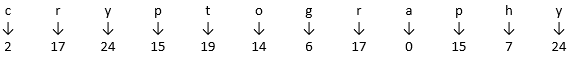
\includegraphics[scale=1]{Table1.PNG}
\end{figure}

As the key was also generated in the form of characters, it too must be converted to a sequence of numbers:

\begin{figure}[H]
\centering
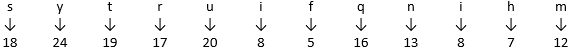
\includegraphics[scale=1]{Table2.PNG}
\end{figure}

Afterwards, the key and the plaintext are added together utilizing modular addition. Of course, all operations below are performed in \textit{mod 26}. Finally, the resulting numbers are converted to the character to which they correspond in the latin alphabet. The resulting sequence of characters is referred to as the ciphertext.

\begin{figure}[H]
\centering
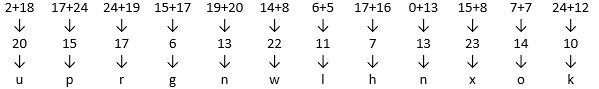
\includegraphics[scale=1]{Table3.PNG}
\end{figure}

\subsection{decoding of the ciphertext using the key}
Assuming the message has been delivered to the intended recipient, who must hold a copy of the secret key (which, as OTP is a symmetrical cryptographical method, is identical to the one utilized to create the ciphertext), the recipient can now decode the ciphertext in order to view the plaintext.

Since the ciphertext was created through the modular addition of the plaintext and the key, the recipient can utilize modular subtraction in order to view the plaintext. In order to do this, the recipient must subtract the key from the ciphertext in modulo 26, and convert the resulting numbers to Latin characters.  However, it is now also necessary for the numbers not to become negative. Fortunatley, this is also made possible by modular arithmetic, as the values simply loop back around from 0 as well. Once again, all below operations are in \textit{mod 26}.

\begin{figure}[H]
\centering
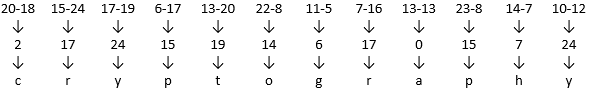
\includegraphics[scale=1]{Table4.PNG}
\end{figure}

Now, the message's journey is complete, having passed from plaintext into ciphertext, being transported to its intended recipient in the form of ciphertext, and finally being decoded and read by its recipient. 

\section{Perfect secrecy: Information-theoretical security}

\subsection{definition}

%\subsection{mathematical proof}

\subsection{Why can only OTP achieve perfect secrecy?}

\section{Issues with OTP}

\subsection{True randomness in generating the key}

\subsection{Secure distribution of the key itself}

\subsection{Secure disposal of a utilized key}


\printbibliography

\end{document}


